\begin{figure}[t!]\center
	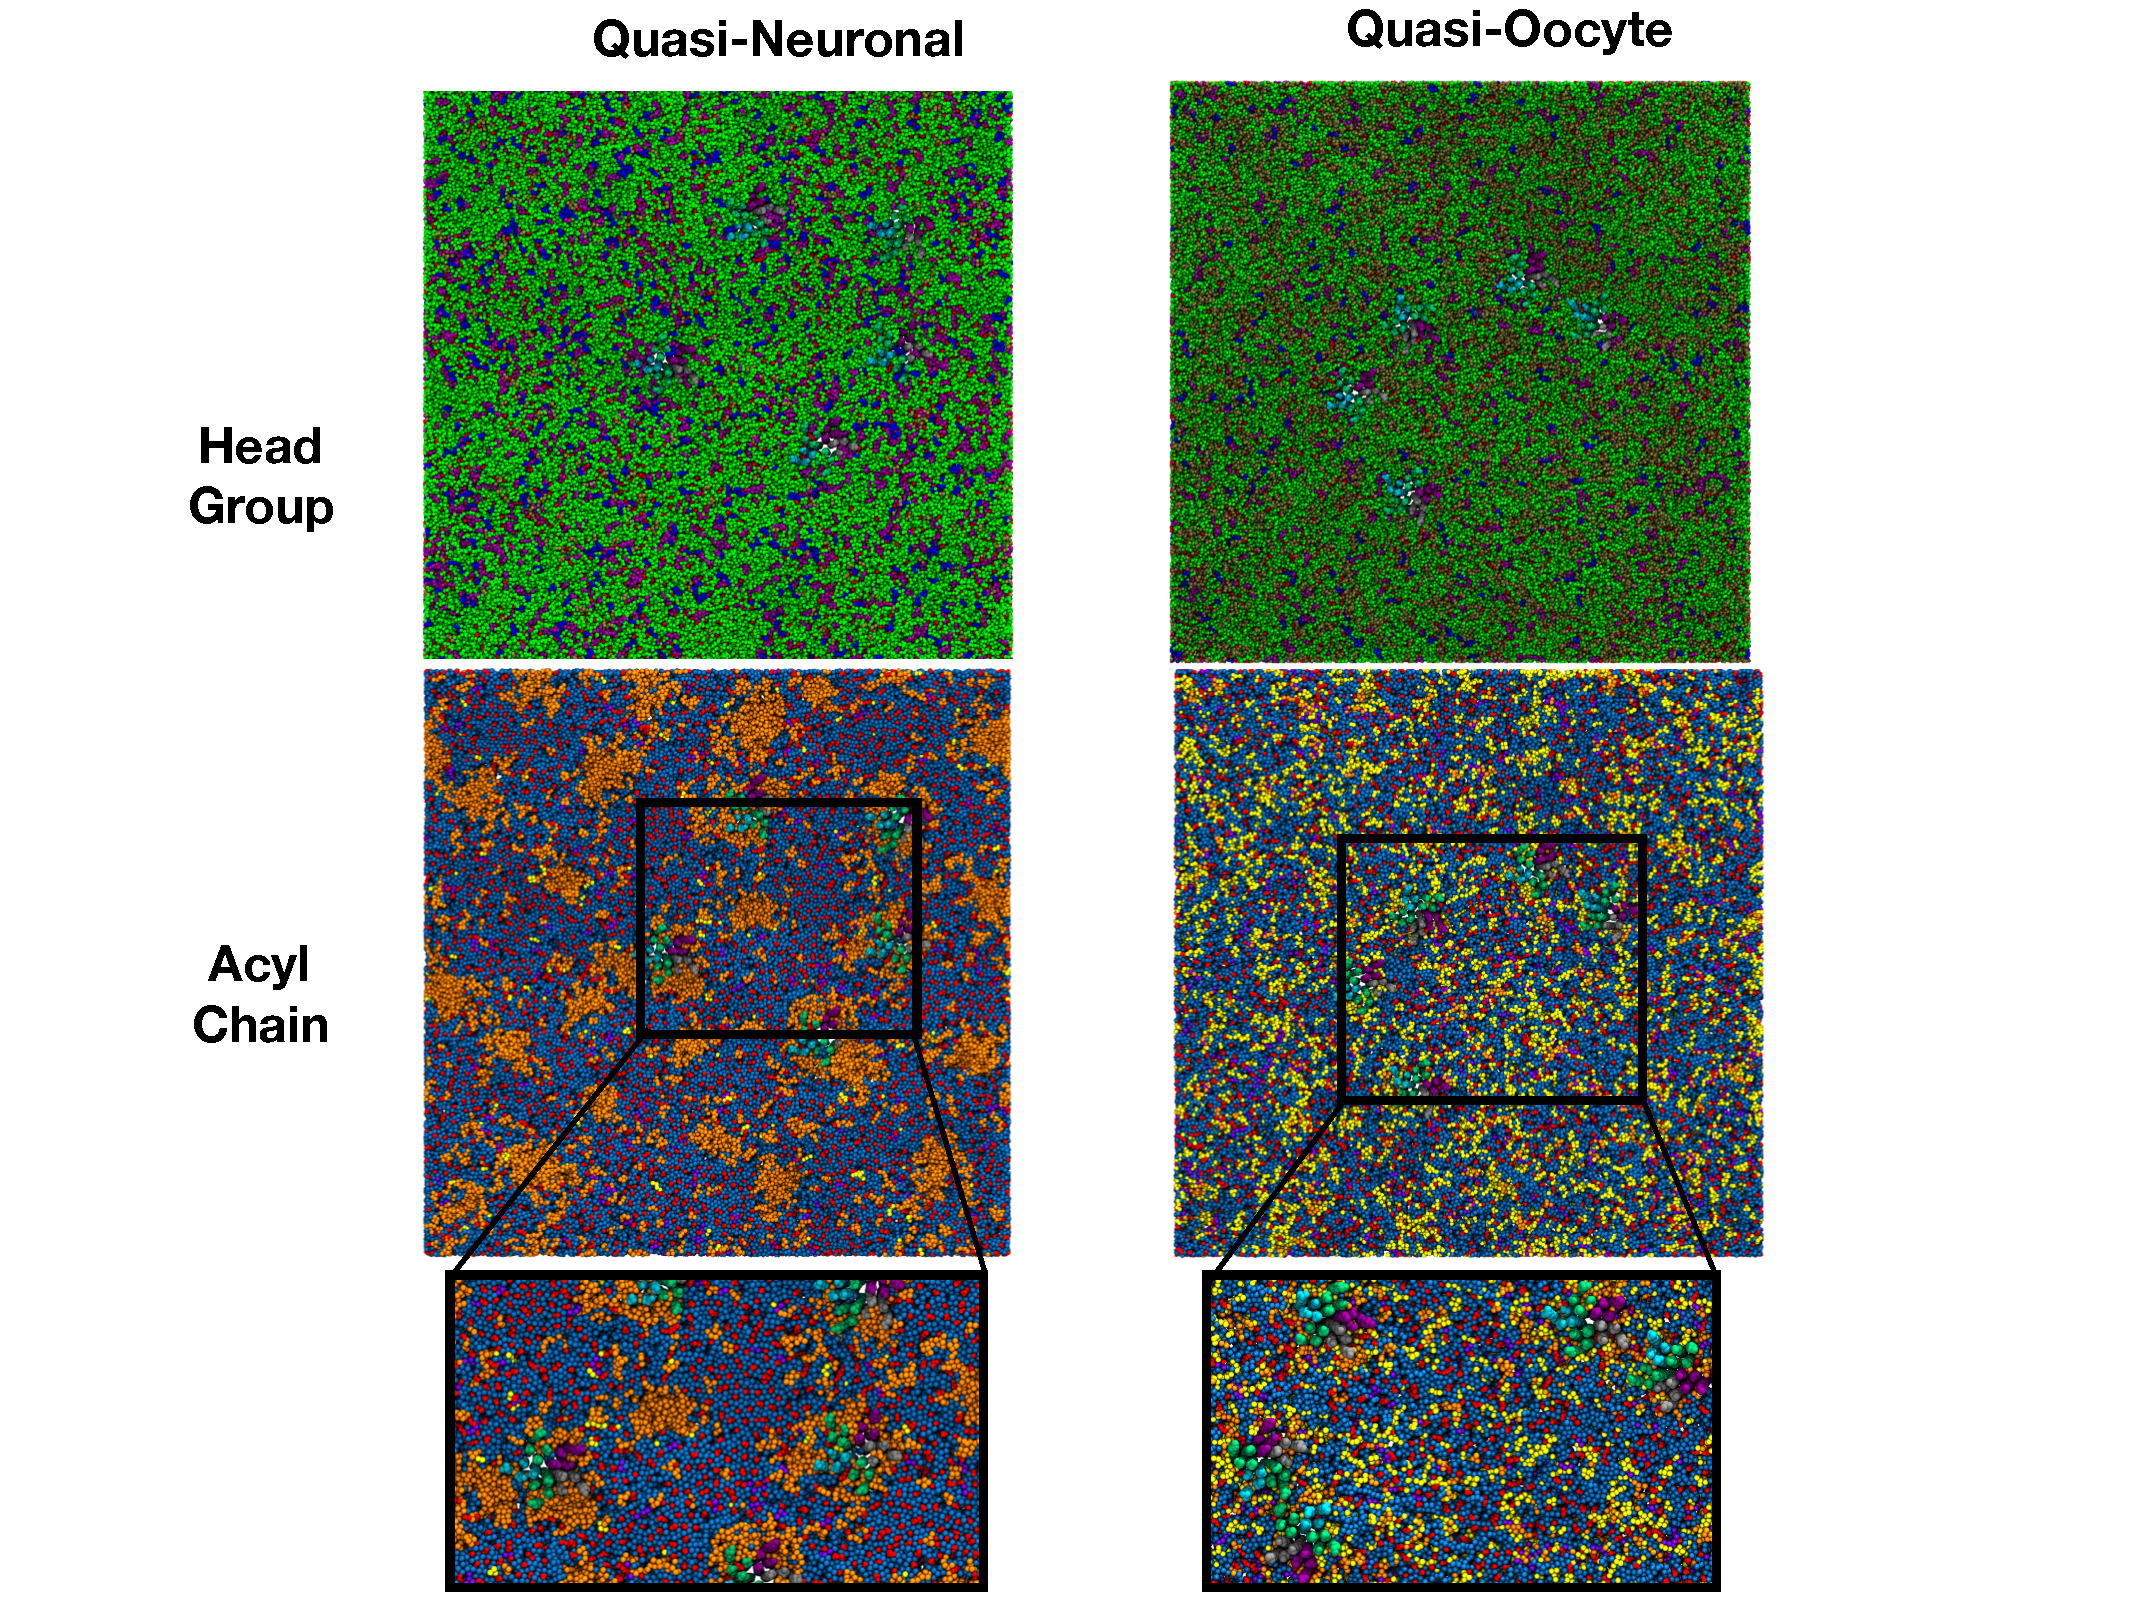
\includegraphics[width=1\linewidth]{./Images/Memb_Comp.pdf}
	\caption{Comparison of nAChR lipid sorting in quasi-Neuronal and quasi-Xenopus oocyte membranes, colored according to either phospholipid head-group or location of acyl chain unsaturation, from coarse-grained MD simulations. nAChR transmembrane domain is shown in surface representation, colored by subunit. Top row: PE (purple), PC (green), SM (tan), PS (blue), cholesterol (red). Bottom Row: n-3 (white), n-6 (yellow), n-9 (purple), saturated (blue), cholesterol (red). Composition of quasi-Neuronal and quasi-Oocyte membranes reflects all species that are sufficiently abundant to yield at least 2 molecules in a membrane of the simulated size. Both systems are fun for $\sim$ 1.5 $\mu s$}
	\label{fig:ooct}
\end{figure}

We observe nAChR partitioning into  n-3 polyunsaturated fatty acid (PUFA)  rich domains with the n-3 PUFA DHA-PE as nAChR's primary boundary lipid. The concentration of n-3 lipids is much lower in membranes, such as Xenopus oocytes,  commonly used in electrophysiology experiments, than in native membranes. I hypothesize adding small concentrations of n-3 is likely to restore the native boundary lipids. I will model various n-3 supplemented quasi-physiological membranes (such as oocytes) to predict those likely to provide a native local environment within the non-native membrane.

pLGICs have complex gating behavior and structural requirements, and nAChRs are some of the most complex pLGICs. One of the most poorly understood components of nAChR is its unpredictable functional sensitivity to slight changes in its lipid environment, a property shared to a lesser extent by other pLGICs \cite{M.CriadoH.Eibl1982,Conti2013}.

Considerable experimental effort \cite{Fong_Correlation_1986,Sunshine_Lipid_1992,Hamouda_Assessing_2006,Butler_FTIR_1993,Bhushan_Correlation_1993,Fong_Stabilization_1987,Corrie_Lipid_2002} was expended, primarily in the 1980s and 1990s, to understand the underlying mechanism of nAChR lipid sensitivity, including identifying the likelihood of specific boundary lipids. Experimental studies focused primarily on cholesterol, which were required in native membranes (20-40\% of lipid composition) to support native levels of ion flux in purified and reconstituted nAChR \cite{Fong_Correlation_1986,Fong_Stabilization_1987}. Further experiments showed that while cholesterol could be depleted from the bulk membrane, a second pool of cholesterol could not be removed from nAChR-containing membranes by depletion \cite{Leibel1987}. However, results were inconclusive regarding whether cholesterol was sufficient to restore nAChR function. Interestingly, soybean lipids (which are also high in n-3 PUFAs) \cite{Yoshida1986,Regost2003,Olsen2003} are more effective at restoring ion flux than cholesterol alone \cite{Morales2006}.

%\begin{figure}[t!]\center
%	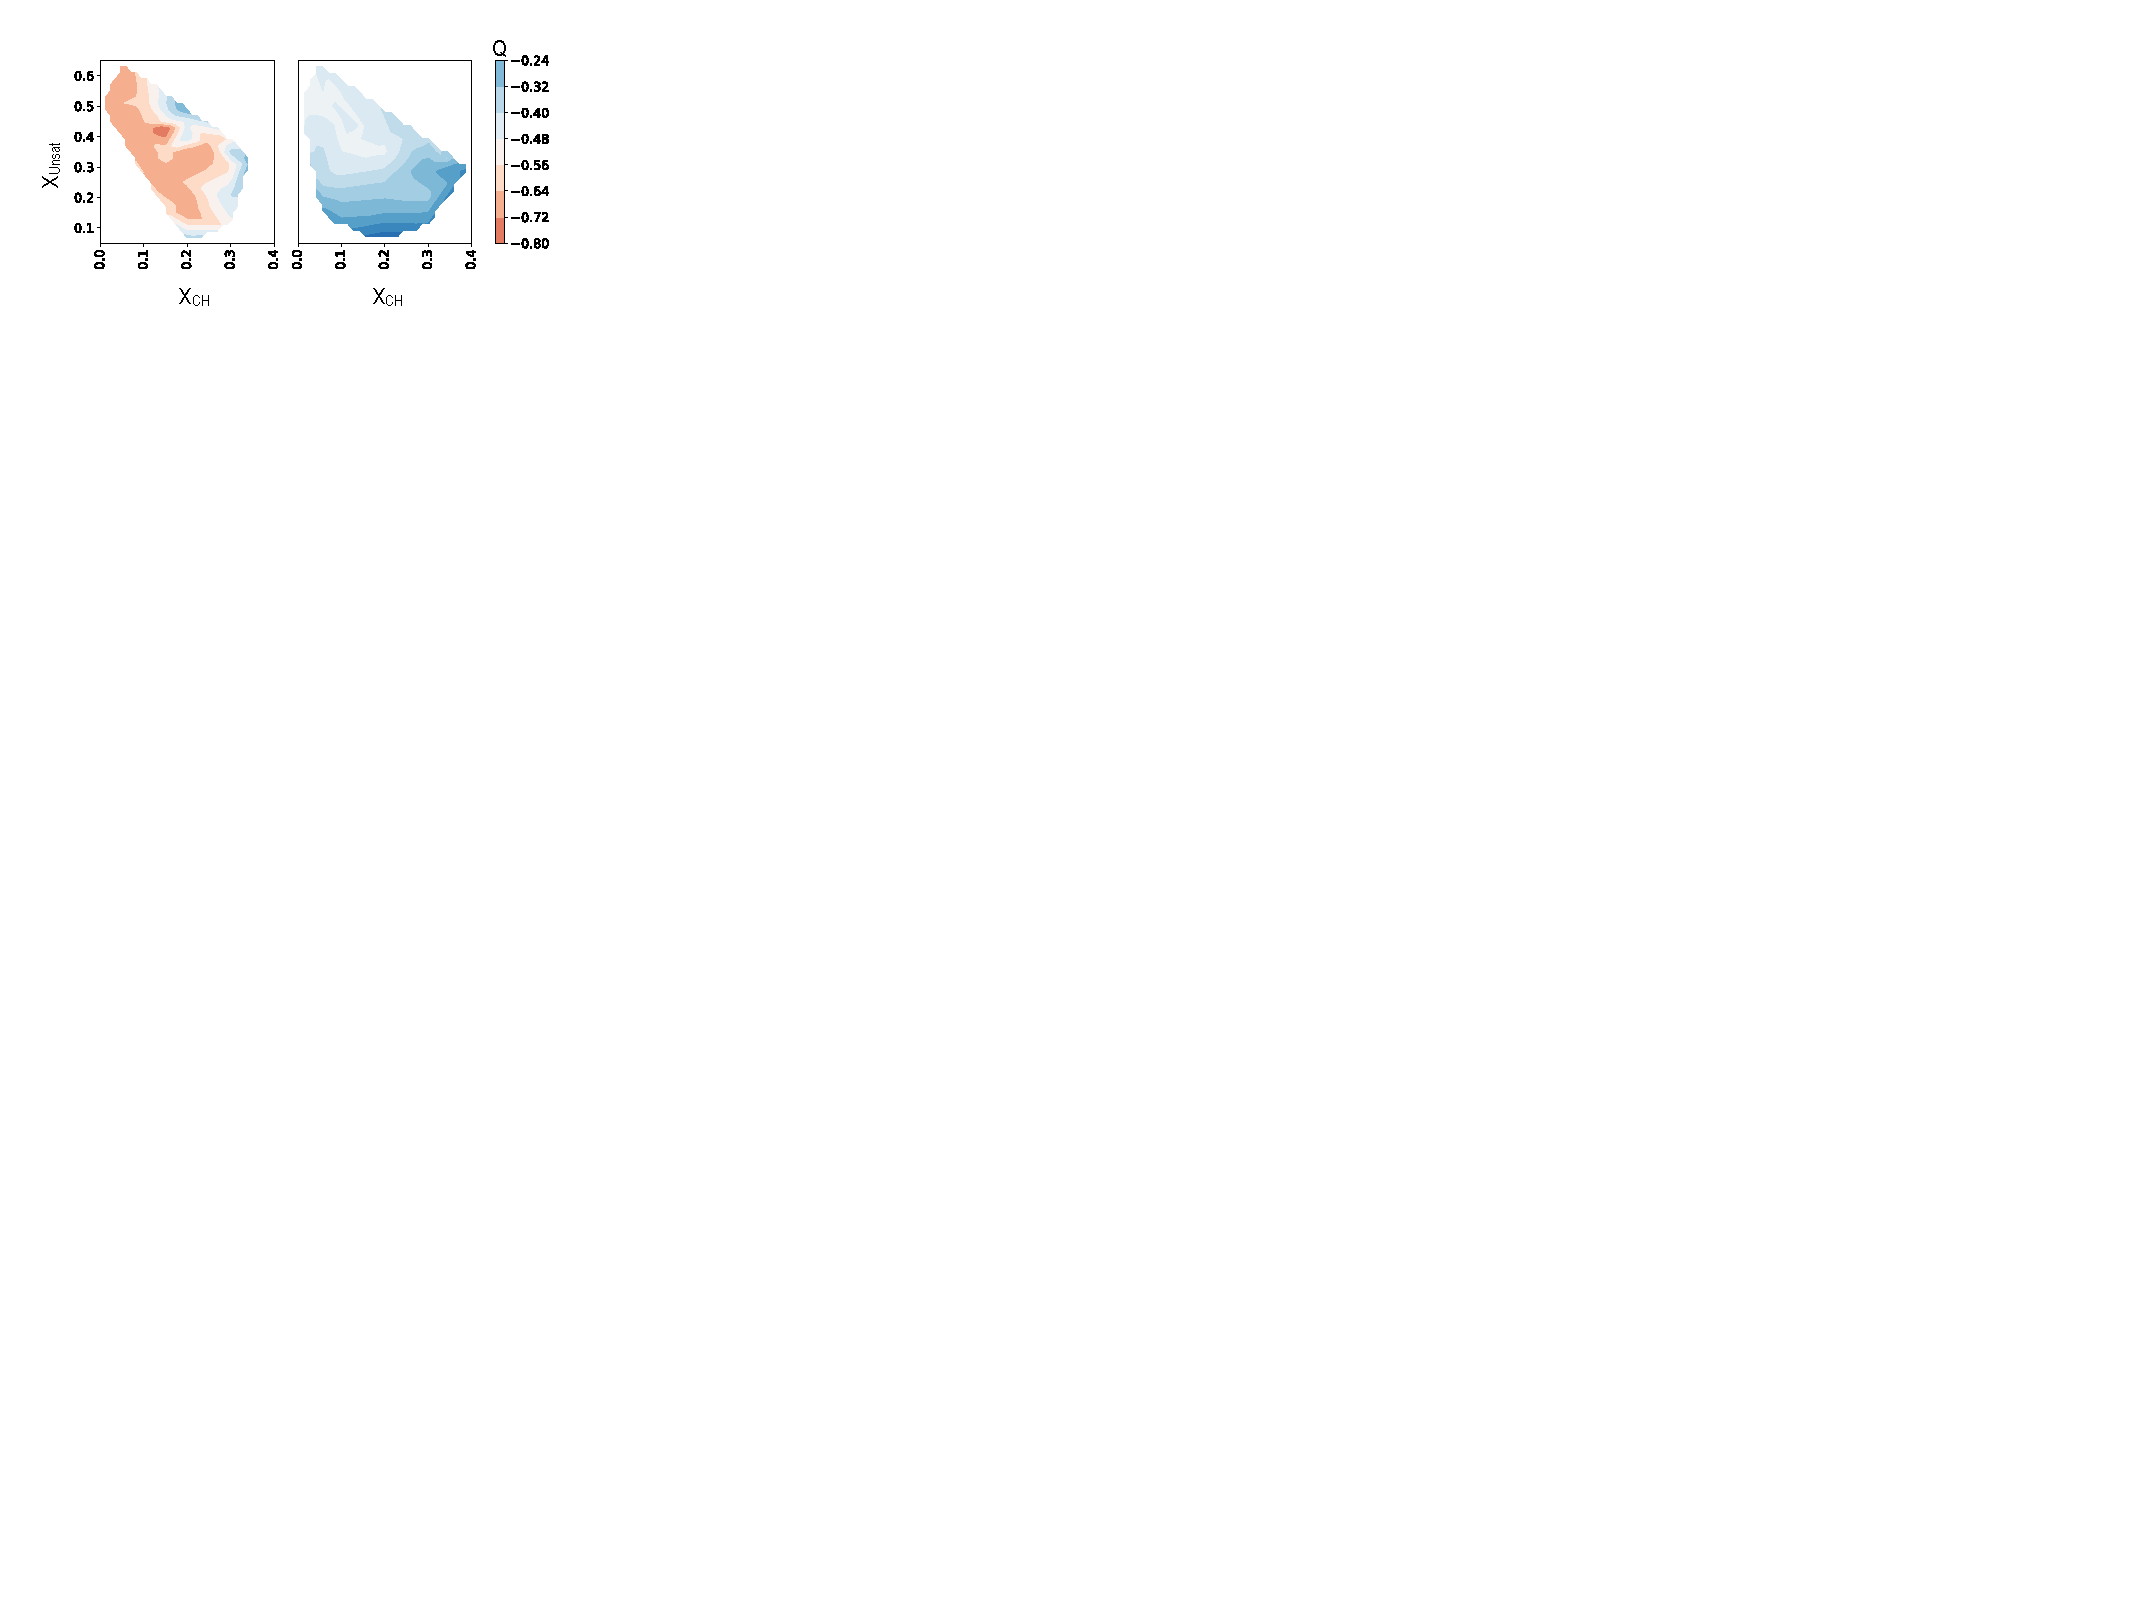
\includegraphics[width=1\linewidth]{./F31/Q.pdf}
%	\caption{Enrichment of nAChR annular lipids for saturated phospholipids in ternary mixture of cholesterol, saturated, and unsaturated phospholipids. $\qsat\equiv \frac{1}{\xsat}\left\langle\frac{  \bsat }{\nbound }\right\rangle-1$, where $\langle bsat\rangle_{\nbound}$ is the averaged fraction of boundary lipids composed of saturated phospholipids, $N_B$ is the total number of boundary lipids, and $\xsat$ is the bulk mole fraction of saturated phospholipid chains. $Q>0$ indicates nAChR preference for the $l_o$ domain; $Q<0$ indicates nAChR preference for the $l_{do}$ domain.}
%	\label{fig:Q}
%\end{figure}

The working assumption in the time of most of those experiments was that the membrane was randomly mixed in the absence of protein, although lipid sorting by proteins was considered likely; there was little evidence available then that cholesterol by itself can induce non-random mixing and even domain formation in just a ternary lipid mixture. We are now also aware of the critical role of acyl chain unsaturation in this process, but previous experiments focused primarily on the role of cholesterol and phospholipid headgroup without including the lipids with n-3 PUFA chains that are so abundant in both the fish electric organ and the postsynaptic membrane.

It is still unknown what factors determine the lipids interacting directly with pLGICs , leading to a substantial source of uncertainty in present-day experiments and introducing a divergence between simulations and experiments that cannot be reasonably estimated. Ionic flux of reconstituted neuronal $\alpha$3$\beta$4nAChR expressed in Xenopus oocytes is less than 50\% of those expressed in mouse-fibroblasts, with neither consistently reproducing native behavior \cite{Fong_Correlation_1986,Sunshine_Lipid_1992,Hamouda_Assessing_2006,Butler_FTIR_1993,Bhushan_Correlation_1993,Fong_Stabilization_1987,Bednarczyk_Transmembrane_2002,Corrie_Lipid_2002}. Contrasts in membrane lipids may contribute significantly to these differences, and specific lipid incorporation may bypass the need for microtransplantation of entire sections of neuronal membranes \cite{Conti2013} into oocytes to achieve native function.
%It is still unknown what factors determine the lipids interacting directly with pLGICs , leading to a substantial source of uncertainty in present-day experiments and introducing a disparity between simulations and experiments that cannot be reasonably estimated. Conductance of recombinant neuronal a3b4nAChR expressed in Xenopus oocytes is less than 50\% of those expressed in mouse-fibroblasts, with neither consistently reproducing native behavior. [34] Differences in membrane lipids may contribute significantly to these differences, and rational lipid supplementation may forgo the need for microtransplantation of entire sections of neuronal membranes[35] into oocytes to achieve native function.

%\subsubsection{Innovation}

A large number of experiments, ranging from the straightforward to the particularly sophisticated, have been carried out to investigate the mechanisms underlying cholesterol modulation of pLGICs. The proposed studies involve investigation of lipid interactions with nAChR via coarse grained molecular dynamics. Numerous simulations of nAChR and other pLGICs with atomic resolution, powerful methods for investigating direct interactions of receptors with small molecules, are also reported in the literature. In the absence of realistic estimates for the protein-local lipid composition, most such simulations embed the receptor in a model membrane composed of DOPC or POPC, with occasional inclusion of cholesterol.

My preliminary studies, which use CG simulations capable of equilibrating a quasi-native membrane, indicate that nAChR has a surprisingly strong preference for n-3 PUFAs (Figures \ref{fig:ooct} and \ref{fig:fig2}B) as boundary lipids. Although these lipids are abundant in most native nAChR membranes, including the electric organ, they had not been included in experiments (except via an abundance in soybean lipids). This surprising observation, if true, offers possible explanations for limited success of many previous experiments.

It further suggests that regardless of the bulk membrane composition, nAChR functions natively in a homogeneous local environment of n-3 PUFAs. Our proposal for reproducing native boundary lipids within an oocyte relies on both this simplicity and the large difference in abundance of n-3 PUFAs between the oocyte and the neuron, which suggests there is a qualitative difference in lipid environment. Microtransplantation of neuronal cell membranes into oocytes \cite{Conti2013} has been carried out and shown to improve ion flux through nAChRs embedded in oocyte membranes, but I will run calculations to inform an approach which restricts supplementation to a few species of preferred boundary lipid, and would substantially improves experimental control. These predictions will be tested by a collaborator of Dr. Brannigan’s, Dr. John Baenziger at University of Ottawa.

%\subsubsection{Approach}

I propose a series of simulations characterizing the boundary lipids surrounding nAChR embedded within a modified oocyte membrane, with the aim of finding the modifications which will reproduce native boundary lipids. %Our initial simulation results suggests nAChR partitions into $l_{do}$ with long chained PUFAs as boundary lipids (see Figure \ref{fig:ooct} and \ref{fig:fig2}B).

The proposed simulations will involve quasi-Oocyte lipid membranes and supplementing them with boundary lipids found in neuronal membranes. I will, first perform literature searches prudent to neuronal/synaptic, \textit{Xenopus} oocyte, and \textit{Torpedo} electric organ membrane compositions. If detailed compositions are not available, I will construct an acyl chain to acyl chain randomizer, to cover all potential lipid species. Constructing a spread sheet (Microsoft Excel) or program (in python), compare and select appropriate Martini equivalent lipids, based on acyl chain length and saturation. Having built a complementary selection of lipids, I will implement automation to allow for easy lipid to membrane supplementation. As there are various n-3 PUFAs, I will construct various series to test which neuronal/\textit{Torpede} n-3 lipid species best assist with native like nAChR boundary domains.

%Differences in the local lipid environments surrounding pLGIC when expressed in common lines for cultured cells will be obtained by computational microscopy; embedding nAChRs in membranes approximating various cell lines including post-synaptic membranes, and \textit{Xenopus} oocytes \cite{Lindi2001,Gamba2005}. 

It is possible (especially if elastic effects are essential) that increasing the number of receptors or the system size will modify these distributions. It is important then, to increase the number of receptors (aiming at around ten), enforcing realistic leaflet asymmetry, and incorporating the newer $\alpha$4$\beta$2 nAChR structure \cite{Morales-Perez_X_2016}. 
%Must be a better way to write this..
%Differences in the local  environment of the pLGIC when expressed in common lines for cultured cells will be obtained by computational microscopy of nAChRs in membranes approximating native membranes, including post-synaptic membranes, as well as common expression systems including Xenopus oocytes[57]. 

%It is possible (especially if elastic effects are essential) that increasing the number of receptors or the system size will modify these distributions. %Therefore, the first step of this aim is improving realism of the simulations of nAChR in the neuronal membrane,
%It is important then, to increase the number of receptors (aiming at around ten), enforcing realistic leaflet asymmetry, and incorporating the newer $\alpha$4$\beta$2 nAChR structure \cite{Morales-Perez_X_2016}. 

%Assuming differences in boundary lipids are maintained, the expression system membrane will have its composition iteratively adjusted to mimic supplementation via liposomes, then allowed to re-equilibrate the local lipid concentration around the receptor.

Currently, I envision an initial analysis of these simulations by calculating membrane mixing, boundary lipid composition, and lipid-protein non-annular binding. Due to the variety of lipid species involved, calculations will be grouped into two sets: lipid head group (i.e. PC, PE, PS...), and acyl chain saturation (i.e. sat, n-1, n-2, n-3, n-6). Preliminary simulations show n-3 dominate the boundary lipids when lipids with n-3 acyl chains are increased by concentrations as low as $\sim$5\%. These initial simulations, quasi-ooctyes with DHA increased to 15$\%$, show DHA to make the dominant boundary lipid. Figure \ref{fig:ooct} shows two of these simulations, using five proteins in quasi-neuronal and quasi-oocyte membranes, and composition asymmetry (albeit mammalian concentration asymmetry). While I have focused on DHA, both n-3 PUFAs, Eicosapentaenoic acid (EPA) and $\alpha$-Linolenic acid (ALA), should also be considered for oocyte modulation.

Once a prediction has been developed for supplementation that would preserve boundary lipids, it will be shared with an experimental collaborator of Dr Brannigan’s, Dr. John Baenziger, to be tested for improved nAChR function. If differences in boundary lipids are not observed, an enrichment protocol will be predicted for shifting the membrane viscoelastic properties to that of the native system.